%----------
%   WARNING
%----------

% This Guide contains Library recommendations based mainly on APA and IEEE styles, but you must always follow the guidelines of your TFG Tutor and the TFG regulations for your degree.

% THIS TEMPLATE IS BASED ON THE IEEE STYLE 

% TFG - Machine Learning Based Predictive Modeling of Energy Prices

%----------
% DOCUMENT SETTINGS
%----------

\documentclass[12pt]{report} % font: 12pt

% margins: 2.5 cm top and bottom; 3 cm left and right
\usepackage[
a4paper,
vmargin=2.5cm,
hmargin=3cm
]{geometry}

% Paragraph Spacing and Line Spacing: Narrow (6 pt / 1.15 spacing) or Moderate (6 pt / 1.5 spacing)
\renewcommand{\baselinestretch}{1.15}
\parskip=6pt

% Color settings for cover and code listings 
\usepackage[table]{xcolor}
\definecolor{azulUC3M}{RGB}{0,0,102}
\definecolor{gray97}{gray}{.97}
\definecolor{gray75}{gray}{.75}
\definecolor{gray45}{gray}{.45}

% PDF/A -- Important for its inclusion in e-Archive. PDF/A is the optimal format for preservation and for the generation of metadata: http://uc3m.libguides.com/ld.php?content_id=31389625.

% In the template we include the file OUTPUT.XMPDATA. You can download that file and include the metadata that will be incorporated into the PDF file when you compile the memoria.tex file. Then upload it back to your project.
\usepackage[a-1b]{pdfx}

% LINKS
\usepackage{hyperref}
\hypersetup{colorlinks=true,
	linkcolor=black, % links to parts of the document (e.g. index) in black
	urlcolor=blue} % links to resources outside the document in blue

% MATH EXPRESSIONS
\usepackage{amsmath,amssymb,amsfonts,amsthm}

% Character encoding
\usepackage{txfonts} 
\usepackage[T1]{fontenc}
\usepackage[utf8]{inputenc}

% English settings
\usepackage[english]{babel} 
\usepackage[babel, english=american]{csquotes}
\AtBeginEnvironment{quote}{\small}

% Footer settings
\usepackage{fancyhdr}
\pagestyle{fancy}
\fancyhf{}
\renewcommand{\headrulewidth}{0pt}
\rfoot{\thepage}
\fancypagestyle{plain}{\pagestyle{fancy}}

% DESIGN OF THE TITLES of the parts of the work (chapters and epigraphs or sub-chapters)
\usepackage{titlesec}
\usepackage{titletoc}
\titleformat{\chapter}[block]
{\large\bfseries\filcenter}
{\thechapter.}
{5pt}
{\MakeUppercase}
{}
\titlespacing{\chapter}{0pt}{0pt}{*3}
\titlecontents{chapter}
[0pt]                                               
{}
{\contentsmargin{0pt}\thecontentslabel.\enspace\uppercase}
{\contentsmargin{0pt}\uppercase}                        
{\titlerule*[.7pc]{.}\contentspage}                 

\titleformat{\section}
{\bfseries}
{\thesection.}
{5pt}
{}
\titlecontents{section}
[5pt]                                               
{}
{\contentsmargin{0pt}\thecontentslabel.\enspace}
{\contentsmargin{0pt}}
{\titlerule*[.7pc]{.}\contentspage}

\titleformat{\subsection}
{\normalsize\bfseries}
{\thesubsection.}
{5pt}
{}
\titlecontents{subsection}
[10pt]                                               
{}
{\contentsmargin{0pt}                          
	\thecontentslabel.\enspace}
{\contentsmargin{0pt}}                        
{\titlerule*[.7pc]{.}\contentspage}


% Tables and figures settings
\usepackage{multirow} % combine cells 
\usepackage{caption} % customize the title of tables and figures
\usepackage{floatrow} % we use this package and its \ ttabbox and \ ffigbox macros to align the table and figure names according to the defined style.
\usepackage{array} % with this package we can define in the following line a new type of column for tables: custom width and centered content
\newcolumntype{P}[1]{>{\centering\arraybackslash}p{#1}}
\DeclareCaptionFormat{upper}{#1#2\uppercase{#3}\par}
\usepackage{graphicx}
\graphicspath{{imagenes/}} % Images folder

% Table layout for engineering
\captionsetup*[table]{
	format=upper,
	name=TABLE,
	justification=centering,
	labelsep=period,
	width=.75\linewidth,
	labelfont=small,
	font=small
}

% Figures layout for engineering
\captionsetup[figure]{
	format=hang,
	name=Fig.,
	singlelinecheck=off,
	justification=centering, % added for formatting consistency
	labelsep=period,
	labelfont=small,
	font=small		
}

% FOOTNOTES
\usepackage{chngcntr} % continuous numbering of footnotes
\counterwithout{footnote}{chapter}

% CODE LISTINGS 
% support and styling for listings. More information in  https://es.wikibooks.org/wiki/Manual_de_LaTeX/Listados_de_código/Listados_con_listings
\usepackage{listings}

% Custom listing
\lstdefinestyle{estilo}{ frame=Ltb,
	framerule=0pt,
	aboveskip=0.5cm,
	framextopmargin=3pt,
	framexbottommargin=3pt,
	framexleftmargin=0.4cm,
	framesep=0pt,
	rulesep=.4pt,
	backgroundcolor=\color{gray97},
	rulesepcolor=\color{black},
	%
	basicstyle=\ttfamily\footnotesize,
	keywordstyle=\bfseries,
	stringstyle=\ttfamily,
	showstringspaces = false,
	commentstyle=\color{gray45},     
	%
	numbers=left,
	numbersep=15pt,
	numberstyle=\tiny,
	numberfirstline = false,
	breaklines=true,
	xleftmargin=\parindent
}

\captionsetup*[lstlisting]{font=small, labelsep=period}

\lstset{style=estilo}
\renewcommand{\lstlistingname}{\uppercase{Código}}


% REFERENCES 

% IEEE bibliography setup
\usepackage[backend=biber, style=ieee, isbn=false,sortcites, maxbibnames=6, minbibnames=1]{biblatex} % Setting for IEEE citation style, recommended for engineering. "maxbibnames" indicates that from 6 authors truncate the list in the first one (minbibnames) and add "et al." as used in the IEEE style.

\addbibresource{referencias.bib} % The references.bib file in which the bibliography used should be


% MY ADDITIONS
% BLOCK DIAGRAMS
% \usepackage{tikz}
% \usetikzlibrary{shapes.geometric, arrows.meta, positioning}

\usepackage{tikz}
\usetikzlibrary{positioning, shapes.geometric, arrows.meta, fit}  % Ensure 'fit' is included

\tikzstyle{process} = [rectangle, minimum width=3.5cm, minimum height=1cm, text centered, draw=black, fill=blue!10] % Maybe get rid of the blue
\tikzstyle{arrow} = [thick,->,>=Stealth]

% INDENT FIRST PARAGRAPH AFTER SECTION
\usepackage{indentfirst}

% CODE - https://www.overleaf.com/learn/latex/Code_listing
\usepackage{listings}

% GANTT DIAGRAM
\usepackage{pgfgantt}
% \usepackage[margin=1in]{geometry} % better margins?

% For top or lower notation in text like 14th
\usepackage{textcomp}

%----------
%	DOCUMENT
%----------

\begin{document}
\pagenumbering{roman} % Roman numerals are used in the numbering of the pages preceding the body of the work.



%----------
%	COVER
%----------	
\begin{titlepage}
	\begin{sffamily}
	\color{azulUC3M}
	\begin{center}
		\begin{figure}[H] % UC3M Logo
			\makebox[\textwidth][c]{\includegraphics[width=16cm]{logo_UC3M.png}}
		\end{figure}
		\vspace{2.5cm}
		\begin{Large}
			University Degree in Telematics Engineering\\			
			 2024-2025\\ % Academic year
			\vspace{2cm}		
			\textsl{Bachelor Thesis}
			\bigskip
			
		\end{Large}
		 	{\Huge ``Machine Learning-Based Predictive Modeling of Energy Prices''}\\
		 	\vspace*{0.5cm}
	 		\rule{10.5cm}{0.1mm}\\
			\vspace*{0.9cm}
			{\LARGE Rodrigo De Lama Fernández}\\ 
			\vspace*{1cm}
		\begin{Large}
			Emilio Parrado Hernández\\
			Madrid, España, May 31st 2025\\
		\end{Large}
	\end{center}
	\vfill
	\color{black}
	% IF OUR WORK IS TO BE PUBLISHED UNDER A CREATIVE COMMONS LICENSE, INCLUDE THESE LINES. IS THE RECOMMENDED OPTION.
	
\includegraphics[width=4.2cm]{creativecommons.png}\\ % Creative Commons Logo
    This work is licensed under Creative Commons \textbf{Attribution – Non Commercial – Non Derivatives}
	\end{sffamily}
\end{titlepage}

%- three spaces will mean next page

\newpage % blank page
\thispagestyle{empty}
\mbox{}



%----------
%	ABSTRACT AND KEYWORDS 
%----------
% summary es algo mas extendido - miro lo que diga la uni
\renewcommand\abstractname{\large\bfseries\filcenter\uppercase{Summary}}
\begin{abstract}
\thispagestyle{plain}
\setcounter{page}{3}
	
	% Write your abstract
    This project focuses on the development of a machine learning-based predictive model for electricity prices in Spain. Using historical data from the OMIE and technical analysis (TA) indicators, the model aims to accurately forecast hourly energy prices. The study focuses on a single hourly slot, evaluating the performance of various Machine Learning models, such as linear regression, Lasso, and Random Forest. There was a strong focus on the feature engineering, employing technical analysis indicators such as moving averages, exponential moving averages, and momentum metrics. The results display the impact of tailoring the features to improve model accuracy and offer insights into the potential of data-driven approaches for energy price forecasting.

% \vspace*{length}
% \medskip
\bigskip
	\textbf{Keywords:} % add the keywords
            
            Energy
            
            Machine Learning
            
            Sliding Window

            Technical Analysis (TA)

            % Add more keywords
            
            % NOT RELEVANT
            % o	Forecasting
            % o	Predictive Modeling
            % o	Neural networks
	
	\vfill
\end{abstract}



\newpage % Blank page
\thispagestyle{empty}
\mbox{}



%----------
%	Dedication
%----------	
\chapter*{Dedication}

\setcounter{page}{5}

% Write here
\noindent Dedicated to my late grandfather, who was not able to see me become an engineer like himself.\\
To my amazing family.\\
To my parents, that have always helped me push through hard moments.\\
To my grandparents who will proudly see me become an engineer.\\
To my amazing girlfriend that has supported me though all the ups and downs of life.\\
To my all of friends and colleagues that have accompanied me these years.\\
To anyone and everyone that has supported me during my years in university.\\

\noindent Here is to the next steps in life

	\vfill



\newpage % blank page
\thispagestyle{empty}
\mbox{}



%----------
%	TOC
%----------	

\tableofcontents
\thispagestyle{fancy}

%--- Estructura TFG (basada en tesis de mama)

    % Agradecimientos
    
    % Dedicatorias
    
    % Indice
    % -	Abstract of the research
    % -	Key words
    
    % 1.	Introduction
    % o	Why am I doing this 
    % 	Personal
    % 	Professional
    % 2.	Marco teorico
    % a.	Teoría de los modelos preditivos
    % b.	Otros estudios
    % c.	Que tipos de modelos hay (y explicar la teoría de los distintos tipos, buscando otros autores que hayan hecho estudios con dichas metodologías y citándolos)
    % i.	Technical Analysis to create a Machine Learning model (24 in parallel)
    % ii.	Time Series Forecasting
    % iii.	Neural Networks
    % 3.	MI Modelo para predecir el precio de la electricidad
    % a.	Metodologia
    % b.	Objeto de estudio
    % c.	Plan de investigación (not really pero valorar)
    % i.	objetivos
    % ii.	preguntas
    % iii.	metodologia
    % 4.	Analysis and Interpretation of the obtained results
    % 5.	Conclusiones de la investigacion y del modelo
    %   a.	Areas de investigación alternativas que se puedan investigar
    % 6.	Referencias Bibliograficas
    % 7.	Glosario de términos
    %   a.	Explicar cosas en detalle
    % 8.	Referencias

%--- Estructura de Emilio

    % Acknowledgements
    
    % Dedication (to… mom dad gf grandparents my teacher etc)
    
    % Index
    % 1.	Introduction
    %     a.	Context (del problema)
    %     b.	Motivation (de la solucion)
    %     c.	Objectives
    %     d.	Summary of the results
    % 2.	Background
    %     a.	Description of the different componentes que uso a modo sencillo - eg modelos etc
    %     b.	ML
    %     c.	Energia
    % 3.	Proposal - si me cambian los datos este capitulo no deberia cambiar
    %     a.	Theoretical system description - esto es como juntas estos componentes - la matriz, el feature selection, los modelos especificos
    %     b. si es una limpieza generica en el tres
    % 4.	Experimentation
    %     a.	Data Description - descripcion de datos y parametros de los resultados - si es una limpieza especifica en el 4
    %     b.	Set Up Explanation - para el RF que rangos de parametros voy a hacer, dias y profundidad, validacion cruzada etc
    %     c.	Results 
    %     d.	Low level discussion
    % 5.	Conclusions
    %     a.	Recap
    %     b.	Revisit Objectives
    %     c.	Future Work
    %           - mejorar el error
%----------



% BLANK PAGE
\newpage % blank page
\thispagestyle{empty}
\mbox{}



%----------
% List of figures. If they are not included, comment the following lines
%----------
\listoffigures
\thispagestyle{fancy}

%     Example of figure:
%     \begin{figure}[H]
%     	\ffigbox[\FBwidth] {
%     	\caption[Name as seen in Index]{Figure name}
%     	}
%     	{
\includegraphics[scale=0.6]{imagenes/creativecommons.png}}
%     \end{figure}

%----------
% List of tables. If they are not included, comment the following lines
%----------
\listoftables
\thispagestyle{fancy}

%     Example of table:
% \begin{table}[H]
% 	\ttabbox[\FBwidth]
% 	{\caption{Lorem ipsum}}
% 	{\begin{tabular}{|c|P{1.5cm}|c|P{1.5cm}|P{2cm}|c|P{1.5cm}|P{2cm}|}
% 		\hline
% 		\multicolumn{2}{|c|}{\textbf{I}} & \multicolumn{2}{c|}{\textbf{II}} & \multicolumn{3}{c|}{\textbf{III}} & \textbf{IV} \\
% 		\hline
% 		x & y & x & y & x & y & x & y \\
% 		\hline
% 		10.0 & 8.04 & 10.0 & 9.14 & 10.0 & 7.46 & 8.0 & 6.58 \\
% 		\hline
% 		8.0 & 6.95 & 8.0 & 8.14 & 8.0 & 6.77 & 8.0 & 5.76 \\
% 		\hline
% 		13.0 & 7.58 & 13.0 & 8.74 & 13.0 & 12.74 & 8.0 & 7.71 \\
% 		\hline
% 		9.0 & 8.81 & 9.0 & 8.77 & 9.0 & 7.11 & 8.0 & 8.84 \\
% 		\hline
% 		11.0 & 8.33 & 11.0 & 9.26 & 11.0 & 7.81 & 8.0 & 8.47 \\
% 		\hline
% 		14.0 & 9.96 & 14.0 & 8.10 & 14.0 & 8.84 & 8.0 & 7.04 \\
% 		\hline
% 		6.0 & 7.24 & 6.0 & 6.13 & 6.0 & 6.08 & 8.0 & 5.25 \\
% 		\hline
% 		4.0 & 4.26 & 4.0 & 3.10 & 4.0 & 5.39 & 19.0 & 12.50 \\
% 		\hline
% 		12.0 & 10.84 & 12.0 & 9.13 & 12.0 & 8.15 & 8.0 & 5.56 \\
% 		\hline
% 		7.0 & 4.82 & 7.0 & 7.26 & 7.0 & 6.42 & 8.0 & 7.91 \\
% 		\hline
% 		5.0 & 5.68 & 5.0 & 4.74 & 5.0 & 5.73 & 8.0 & 6.89 \\
% 		\hline
% 		\multicolumn{5}{l}{Source: BOE}
% 	\end{tabular}}
% \end{table}

%----------
%	THESIS
%----------	
\clearpage
\pagenumbering{arabic} % numbering with Arabic numerals for the rest of the document.	

% IMPORTANT: Latex special characters are: # $ % & \ ^ _ { } ~. To avoid mistakes when compiling try writing \ before. For: \ use \textbackslash ; for ^ \textasciitilde and ~ \textasciicircum.

% Start writing here----------------------------------------------------



% Chapter 1 - introduction to the problem
\chapter{Introduction to the problem}
    \begin{itemize}
    \item \textbf{1. Explanation of how the price of energy works in Spain}
        \begin{itemize}
        \item a. Energy
        \item b. Prices
        \end{itemize}
    \item \textbf{2. Machine Learning - Lets run through some model overviews, which are available to choose, but without actually referencing anything}
    \end{itemize}

% We thought about different approaches such as Time-Series Forecasting, about Neural Networks but ...
Energy has increasingly become more important.
Availability is key for a modern high functioning society
In Europe we are lucky to have a really advanced and reliable network.
It is a key resource needed to succeed in the ecological transition that we are currently undergoing world wide.
Electric mobility is a key element of this process.
Electric cars, buses and trucks, need easily available and convenient sources of energy to recharge, to be able to play their role in society.
An important factor in this ever growing necessity is the price of the available energy.
But in recent times, that easy and affordable access has changed, and has become more unpredictable.
Ever since the commencement of the war between Russia and Ukraine marked and inflection point in the mostly cyclical nature of electricity prices.
Prices have gone up considerable since a couple years time, and it has been affecting everyone, from big consumers such as companies, to everyday people, having to pay a more expensive electricity bill at the end of the month.
This has become a topic of great concern, with more and more people thinking about it often.

This led me to think about pricing, how it was structured, and what to expect as an end consumer.
Could we plan our use of energy according to the price?
Could it be predicted accurately?
These were some of the questions I had that sparked my interest in looking into energy predictions.

In the initial discussions of this project, we talked about various ways to attack the problem at hand.
We thought about a variety of systems but settled on a plan to explore the predictions with the more established methods of Machine Learning.
This was done specially since it was a natural continuation of what was learned in the third year subject of Telematics Engineering, Modern Theory of Detection and Estimation.

The first idea we developed was to separate out the project in 24 blocks, one for each hour block to predict.
The reason behind splitting the data in 24 blocks was simple, we assumed that data between the same time slot across neighbor days, would be similar, or would follow a certain trend.

Focusing on the innovation side of things, we decided to simplify the problem.
Pivoting from creating an algorithm to predict hourly prices, to splitting that into the 24 blocks, and predicting a single one.
We decided on the 14\textsuperscript{th} hour of each day, since irrespective of the day of the week, or holiday, it would always be a valley period.

This kind of granular breaking up of data is similar to what a Random Forest does in order to absorb more details and create higher resolution predictions. We made this assumption based on the idea that it would simplify the project substantially.
% This forced us to generalize our approach, creating a system to analyze and evaluate the data in 24 distinct blocks, figuring out the best matrix dimensions for our linear regression matrix.

Talk about Emilio's background in investment banking at BBVA and his alorithms.

Talk about the idea of using technical analysis for feature engineering



% Chapter 2 - Background and Related Work (State of the Art???)
\chapter{Background and Related work}
% \begin{itemize}
% \item \textbf{References}
%     \begin{itemize}
%         \item How is the price of electricity / energy set? What happens if new producers enter the market?
%         \item Articles that reference energy prices prediction as an inspiration for my own work:
%         \begin{itemize}
%             \item 5-10 articles that do/talk about similar things
%             \item Energy consumption predictions
%             \item Energy prices in other European countries (Italy, Germany, UK, France)
%             \item Longer term predictions
%             \item Predicciones de produccion
%         \end{itemize}
%         \item Describir tecnologias – explicar mas en detalle como funciona y enlaces a donde pueda averiguar el contenido
%     \end{itemize}

%     \item Referenciar que metricas uso para medir mi error etc
%     \item Referencias de donde saco los datos

%     \item Referencias a que software utilizo referencias a documentacion de sklearn etc
% \end{itemize}

\section{General background}
How is the price of electricity set in Spain and Portugal?

LEER ARTICULO \cite{precio_electricidad_edem}


What happens when new producers enter the market and sell to the energy pool?

Comment about more typical case studies focusing on energy consumption, since that is something more consistent and predictable

\section{The Sliding Window plan: Setting up the Feature Matrix}

How do I prepare my data to utilize across different models: The Feature Matrix (weight matrix)

The sliding window theory (mini-models)

\section{Which Machine Learning models will be used}
What algorithms will I use?

- Linear Regression: \url{https://scikit-learn.org/stable/modules/generated/sklearn.linear_model.LinearRegression.html}
% Ordinary least squares Linear Regression.

% LinearRegression fits a linear model with coefficients w = (w1, …, wp) to minimize the residual sum of squares between the observed targets in the dataset, and the targets predicted by the linear approximation.


- Lasso Regression: \url{https://scikit-learn.org/stable/modules/generated/sklearn.linear_model.Lasso.html}
% Linear Model trained with L1 prior as regularizer (aka the Lasso).

% The optimization objective for Lasso is:

% (1 / (2 * n_samples)) * ||y - Xw||^2_2 + alpha * ||w||_1

% Technically the Lasso model is optimizing the same objective function as the Elastic Net with l1_ratio=1.0 (no L2 penalty).


% The algorithm used to fit the model is coordinate descent.

% To avoid unnecessary memory duplication the X argument of the fit method should be directly passed as a Fortran-contiguous numpy array.

% Regularization improves the conditioning of the problem and reduces the variance of the estimates. Larger values specify stronger regularization. Alpha corresponds to 1 / (2C) in other linear models such as LogisticRegression or LinearSVC. If an array is passed, penalties are assumed to be specific to the targets. Hence they must correspond in number.

% The precise stopping criteria based on tol are the following: First, check that that maximum coordinate update, i.e. 
%  is smaller than tol times the maximum absolute coefficient, 
% . If so, then additionally check whether the dual gap is smaller than tol times
% .

% The target can be a 2-dimensional array, resulting in the optimization of the following objective:

% (1 / (2 * n_samples)) * ||Y - XW||^2_F + alpha * ||W||_11

% where 
%  is the sum of the magnitude of the matrix coefficients. It should not be confused with MultiTaskLasso which instead penalizes the 
%  norm of the coefficients, yielding row-wise sparsity in the coefficients.


- Random Forest: \url{https://scikit-learn.org/stable/modules/generated/sklearn.ensemble.RandomForestRegressor.html}
% A random forest regressor.

% A random forest is a meta estimator that fits a number of decision tree regressors on various sub-samples of the dataset and uses averaging to improve the predictive accuracy and control over-fitting. Trees in the forest use the best split strategy, i.e. equivalent to passing splitter="best" to the underlying DecisionTreeRegressor. The sub-sample size is controlled with the max_samples parameter if bootstrap=True (default), otherwise the whole dataset is used to build each tree.

% For a comparison between tree-based ensemble models see the example Comparing Random Forests and Histogram Gradient Boosting models.


\section{Fine Tuning with Technical Analysis and Feature engineering}
What Type of finetuning will I use?

- Feature engineering \& selection

- Technical analysis based feature engineering
    
    TA metrics used? SMA, EMA, ROC \& RSI

    Talk about the intervals used:
    
    $ SMA_3,SMA_5,SMA_7,SMA_{14},SMA_{30},SMA_{60},SMA_{90},SMA_{180},SMA_{360} $
    
    $ EMA_3,EMA_5,EMA_7,EMA_{14},EMA_{30} $
    
    $ ROC_3,ROC_5,ROC_7,ROC_{12},ROC_{14},ROC_{30} $
    
    $ RSI_5,RSI_7,RSI_{14} $

\section{Evaluation Metrics}
How will I measure my accuracy?

errors:

$ R^2 $

RMSE \& MSE

\section{Related Work}
Other ways of predicting

Temporal Series

Energy consumption predictions





% Chapter 3 - Proposal - Theoretical System Description ?
\chapter{Theoretical System Proposal Description}

This chapter will outline the design of the system developed for the project, describing the complete pipeline constructed for the system. This will be explained starting from a blank state, detailing the complete set-up process required to run the project. Following this initial configuration, the data preparation stage will be outlined. This will be continued by the feature matrix creation process, concluding with the training of the machine learning models and the chosen evaluation methods.

The following Block diagram will model in the most basic forms the system design:
%--- (block diagram)

% Retrieve Data from OMIE

% Ingest data and create a CSV DB

% Verify and Clean up the DB

% Create Sliding Window Matrix for use in training that batch

% Train the batch

% Check out predictions of each mini-model with actual energy price for that time slot

% Review error rates and compare with other iterations/ batches and other models.

% SIMPLE DIAGRAM
% \begin{center}
% \begin{tikzpicture}[node distance=1.5cm]

% % Nodes
% \node (retrieve) [process] {Retrieve Data from OMIE};
% \node (ingest) [process, below of=retrieve] {Ingest Data and Create CSV DB};
% \node (clean) [process, below of=ingest] {Verify and Clean up the DB};
% \node (matrix) [process, below of=clean] {Create Sliding Window Matrix};
% \node (train) [process, below of=matrix] {Train the Batch};
% \node (predict) [process, below of=train] {Check Predictions vs Actual Price};
% \node (review) [process, below of=predict] {Review Errors \& Compare Models};

% % Arrows
% \draw [arrow] (retrieve) -- (ingest);
% \draw [arrow] (ingest) -- (clean);
% \draw [arrow] (clean) -- (matrix);
% \draw [arrow] (matrix) -- (train);
% \draw [arrow] (train) -- (predict);
% \draw [arrow] (predict) -- (review);

% \end{tikzpicture}
% \end{center}

% MORE COMPLEX DIAGRAM
\begin{figure}[H]
    \centering
    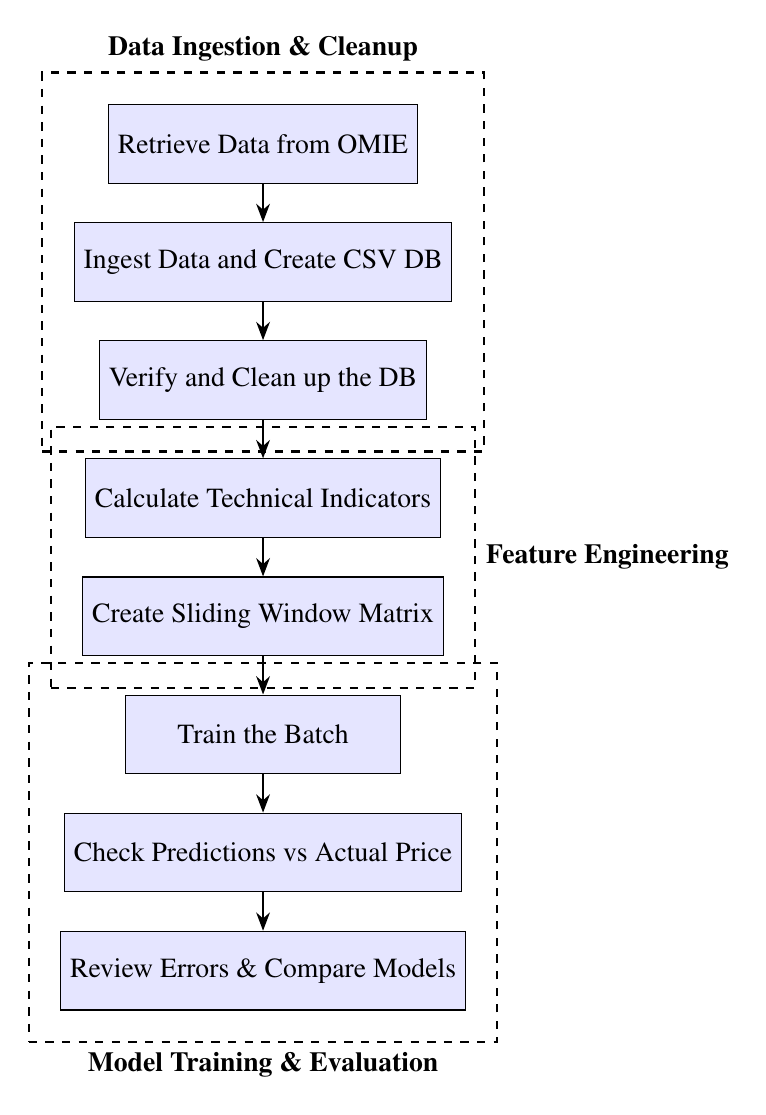
\begin{tikzpicture}[node distance=1.5cm]
    
    % Styles
    \tikzstyle{process} = [rectangle, minimum width=3.5cm, minimum height=1cm, text centered, draw=black, fill=blue!10]
    \tikzstyle{arrow} = [thick,->,>=Stealth]

    % Nodes
    \node (retrieve) [process] {Retrieve Data from OMIE};
    \node (ingest) [process, below of=retrieve] {Ingest Data and Create CSV DB};
    \node (clean) [process, below of=ingest] {Verify and Clean up the DB};
    \node (indicators) [process, below of=clean] {Calculate Technical Indicators};
    \node (matrix) [process, below of=indicators] {Create Sliding Window Matrix};
    \node (train) [process, below of=matrix] {Train the Batch};
    \node (predict) [process, below of=train] {Check Predictions vs Actual Price};
    \node (review) [process, below of=predict] {Review Errors \& Compare Models};

    % Arrows
    \draw [arrow] (retrieve) -- (ingest);
    \draw [arrow] (ingest) -- (clean);
    \draw [arrow] (clean) -- (indicators);
    \draw [arrow] (indicators) -- (matrix);
    \draw [arrow] (matrix) -- (train);
    \draw [arrow] (train) -- (predict);
    \draw [arrow] (predict) -- (review);

    % Group boxes
    \node[draw=black, thick, dashed, fit={(retrieve)(ingest)(clean)}, inner sep=0.4cm, label=above:{\textbf{Data Ingestion \& Cleanup}}] {};
        \node[draw=black, thick, dashed, fit={(indicators)(matrix)}, inner sep=0.4cm, label=right:{\textbf{Feature Engineering}}] {};
    \node[draw=black, thick, dashed, fit={(train)(predict)(review)}, inner sep=0.4cm, label=below:{\textbf{Model Training \& Evaluation}}] {};

    \end{tikzpicture}
    \caption{Theoretical Block Diagram of the Project Pipeline}
    \label{fig:block_diagram_pipeline}
\end{figure}
%--- END (block diagram)

% Three main blocks

% Data ingestion and cleanup
% The Feature Matrix for the Sliding Window Approach
% Training of each model with the Matrix

%--- SUMMARY

Data Preparation

Matrix Creation

Mini-models - sliding window approach

The thought process behind our sliding window approach has to do with the data and the
No estacionario. No son datos IID - Independientes e identicamente distribuidos.
Hay correlacion en mis datos entre cada dia? Si deberia ser relativamente alta, estacional, pero progresiva y lenta.

Technical indicators
Que es cada cosa y porque usarlos en vez de series temporales, porque la info temporal esta implicita en los indicadores.
Indicadores que capturan patrones en la serie
Ventaja: modelo ML mas sencillo pq las features son muy informativas vs

ML blocks
    Linear Regression
        Linear combination of every feature
    Lasso Regression
        Can turn unimportant features into 0s
    Random Forest
        Feature engineering

Pandas, NumPy, scikit-learn

%--- END SUMMARY

Retrieve Data from OMIE

Kick-starting the pipeline design, the data is retrieved from the OMIE website, and is ingested into a CSV file that will act as our rudimentary database. The process is done with the following code:

After a successful retrieval, the database is checked for missing or repeated data points. This will be checked in a time-slot basis.

Since the idea is to cater to any potential system, it was created without any hour slot preference, but in the system I will be proposing, we will limit the dataset to just the 14h time-slot.

The database will be transformed into a reduced set, containing only the relevant data points, measured always at 14h

Subsequently comes the creation of the feature matrix. This will initially consist of exclusively the sliding window width desired for that training batch.

Once the matrix is created (and verified), the training process begins.

Due to our particular system, the training will consist of complete rows of that feature matrix.

Cross validation?? Not really done, in another way w the sliding window
cambio parametros pero no la arquitectura del modelo

Review the mini model theory, why is it reasonable to not use training set, validation and test sets?

Review error rates and compare with other iterations/ batches and other models.

%----------------------------------
\noindent \textbf{Detailed Steps:}

Prior set up:

Developed and tested with Python 3.13 \cite{python}

To set up a new virtual environment \cite{python_venv} run:
\begin{verbatim}
python -m venv .venv
\end{verbatim}

To activate the new virtual environment run:
\begin{verbatim}
in macOS
source .venv/bin/activate
in Windows
.venv\Scripts\Activate.ps1
\end{verbatim}

Install the following contents to reproduce the original virtual environment:
\begin{verbatim}
# To install the following packages run:
# pip install -r requirements.txt 
ipykernel==6.29.5
matplotlib==3.10.1
numpy==2.2.3
pandas==2.2.3
requests==2.32.3
scikit-learn==1.6.1
ta==0.11.0
\end{verbatim}

1. Download of OMIE data (only section independent of the whole system)
\cite{omie_datos}

Downloaded with a Python script for the dates that were not available with an easy .zip file (for whole previous years):

Insert the python script?? better suited for an annex??
\begin{lstlisting}
import requests
from datetime import datetime, timedelta

# Usage instructions:
    # Set file name to save the filenames to download
    # Set start and end dates

file_path = 'to_download.txt'
start_date = datetime(2025, 2, 14)
end_date = datetime(2025, 3, 18)

# Compose filenames to download
def compose_filenames():
    start_date = start_date
    end_date = end_date
    
    # Generate the entries for the number of days comprehended
    to_generate = (end_date - start_date).days + 1
    entries = []
    for i in range(0, to_generate):  # x days from start to end
        date_entry = start_date + timedelta(days=i)
        entries.append(f'marginalpdbc_{date_entry.strftime("%Y%m%d")}.1')
    
    # Save to a .txt file
    with open(file_path, 'w') as file:
        for entry in entries:
            file.write(entry + '\n')

# Example URI to build
# https://www.omie.es/es/file-download?parents%5B0%5D=marginalpdbc&filename=marginalpdbc_20230102.1
def read_filenames_and_compose_urls(file_path):
    base_url = "https://www.omie.es/es/file-download?parents%5B0%5D=marginalpdbc&filename="
    
    # Read the filenames from the .txt file
    with open(file_path, 'r') as file:
        filenames = [line.strip() for line in file if line.strip()]
    
    # Compose the URLs
    urls = [base_url + filename for filename in filenames]
    
    return urls

def download_files(urls):
    for url in urls:
        # Extract the filename from the URL
        filename = url.split('=')[-1]
        
        # Send a GET request to download the file
        # response = requests.get(url)
        response = requests.get(url)
        
        # Check if the request was successful and write to file
        if response.status_code == 200:
            # Write the content to a file with the extracted filename
            with open(filename, 'wb') as file:
                file.write(response.content)
            print(f"Downloaded {filename}")
        else:
            print(f"Failed to download {filename}")

# Execution
compose_filenames()
urls = read_filenames_and_compose_urls(file_path)
download_files(urls)
\end{lstlisting}

2. Data shape? NEXT CHAPTER 4

3. Data format: NEXT CHAPTER 4

4. Data organization

We will transform the data into a CSV format easier to use with the Pandas library to later create a DataFrame. We will maintain the same information, but in a encoding more suitable for Pandas. For that, the date and time must be transformed to a format such as Datetime which will transform the information from \texttt{2018;01;01;14; ...} to \texttt{2018-01-01 14:00:00}

5. Data visualization with Seaborn? With Microsoft Corporation's "Data Wrangler" VSCode extension

6. Data retention of only the relevant info time and date, and MarginalES - drop MarginalPT

7. Data cleanup:
Check for missing or duplicate entries. since Daytime Savings introduces duplicate hours some days of the year:
INSERT some dates in the dataset that have the duplicated entries

8. Explain all blocks of the system?
    Data download:
    Data ingest

Contar los bloques empleados en cada parte – como junto las piezas para construir el sistema – porque uso las piezas que uso

Hablar de implementaciones como que librerías, que scripts etc – no es muy necesario, mas importante la idea
%----------------------------------
% Create three chapters

\section{Data Ingestion}

\section{Matrix Creation}

\section{Model Training}

%----------------------------------



% Chapter 4 - Experimentation
\chapter{Experimentation}
This chapter is dedicated to reviewing all of the relevant information pertaining the experimentation phase of the project. We will review the specifics of the data that was dealt with, and explain the decisions taken for the preparation of such data, and the training of the different machine learning models employed. We will review all of the results of the different models, and discuss in depth the different set-up variations for the models.

\section{Data Description} % Data Description – OMIE data
The data that was used for this project was exlcusively publicly available information, published by the OMIE, which stands for \textit{Operador del Mercado Ibérico de Energía}, meaning the Iberian operator of the energy market. The data that was retrieved for the project takes the following shape:

\begin{small}
\begin{verbatim}
MARGINALPDBC;
2018;01;01;1;28.1;6.74;
2018;01;01;2;33;4.74;
2018;01;01;3;32.9;3.66;
2018;01;01;4;28.1;2.3;
2018;01;01;5;27.6;2.3;
2018;01;01;6;24.6;2.06;
2018;01;01;7;20.1;2.06;
2018;01;01;8;19.9;2.06;
2018;01;01;9;19.84;2.3;
2018;01;01;10;19.9;2.3;
2018;01;01;11;19.9;2.3;
2018;01;01;12;19.9;2.3;
2018;01;01;13;23.6;2.3;
2018;01;01;14;25.1;2.3;
2018;01;01;15;23.6;5;
2018;01;01;16;24.6;5;
2018;01;01;17;25.1;5;
2018;01;01;18;27.6;8.85;
2018;01;01;19;27.6;15.93;
2018;01;01;20;28.1;22.02;
2018;01;01;21;32.9;20;
2018;01;01;22;28.1;21.95;
2018;01;01;23;28.1;23.52;
2018;01;01;24;27.6;16.35;
*
\end{verbatim}
\end{small}

We can understand and interpret this format following the OMIE's guide: \textit{Modelo de Ficheros para la distribución pública de Información del mercado de electricidad 1.35} \cite{omie_formatos_2024}. In page number 67, chapter 6.18 we may find the following information regarding the encoding format for the information:

\begin{small} % so a bit more text can appear
\begin{verbatim}
6.18 Precios marginales del mercado diario (MARGINALPDBC)

Fichero con los precios marginales del Mercado Diario para cada una de
las horas.
Nombre del fichero: marginalpdbc_aaaammdd.v donde aaaammdd
corresponde a la fecha de sesión y v es la versión del fichero.

Descripción de los campos:
CAMPO DESCRIPCIÓN VALORES VÁLIDOS
Año Año I4 – 20XX
Mes Mes I2 – 1 a 12
Día Día I2 – 1 a 31
Hora Hora I2 – 1 a 25
MarginalPT Precio marginal zona Portuguesa F8.2 – -99999.99 a 99999.99
MarginalES Precio marginal zona Española F8.2 – -99999.99 a 99999.99
\end{verbatim}
\end{small}

From this data description we can obtain the following column names: \textit{Año, Mes, Día, Hora, MarginalPT} and \textit{MarginalES}. As a proof of concept, in this investigation we will be focusing on a single time slot, simplifying the data, from multiple data points per day, to a single one. We are exclusively interested in the value of the last column, \textit{MarginalES}, and specifically the row pertaining the 14\textsuperscript{th} hour of each day, which we will refer to as 14H.
% another option 14$^{th}$

For the data visualization portion, I employed various methods, bot plotting values with matplotlib, seaborn and using the Microsoft Data Wrangler Visual Studio Code extension.

Explain some more about the data distribution.

Explain the ups and downs of the data (war and relation to natural gas prices).

Explain the zero price.

\section{Set Up Explanation}
How do I use the previously explained system - what parameters did I modify to obtain the final results. Feature engineering, Alpha variation testing in Lasso, Tree depth and number of leafs.
Que modelos y que configs

- Linear Regressor

- Lasso Regressor

- Random Forest
%como lo usas en el sentido de tocar cosas, parametros como numero de arboles profundidad, el Alpha del lasso

\section{Results of the Testing}
Results as graph/ tables - This would be to compare a model across various iterations. Model best-run comparisons, etc.
% a modo tabla unica comparando todas las iteraciones de cada technologia, y luego una conjunta con la mejor de todo (Si me hace falta mas, pues al apendice)

Error medio en todas las predicciones
Y percentiles (expectation shortfall tambien?)

\section{Low Level Discussion} % of the results
This would be the final explanation that I would give to a colleague of mine, with full details on how I have done everything



% Chapter 5 - Regulatory Framework (Marco Regulador)
\chapter{Regulatory Framework}
Not essential for this investigative project because we do not go to market.

\section{Data Availability}
Habria que hablar de las normas, pq si alguien lo usa es para ir a mercado

Current Spanish and European regulations allow for the use of publicly available institutional data for use in educational investigative work.

I need to talk about laws, what data is permissible to use and how. This would be essential for a project that does indeed go to market.

For us, its not that relevant.

\section{Software \& Licenses}

For the development of this project I have used a variety of open and closed source utilies and code.

For the sake of organization, I will categorize this section into two distinct parts, required software to reproduce the project, and optional software for ease of production, plannification, organization or otherwise related.

Required:

Python - This was the programming language in wich the entirety of the project was developed \cite{python}

Scikit-learn - library for ml \cite{scikit-learn}

Pandas - data management \cite{pandas}

ta library - Technical Analysis library\cite{ta-lib}

Light use of Seaborn - data visualization \cite{seaborn}

NumPy - number manipulation \cite{numpy}

macOS / Windows - closed source platforms across where the project was developed \cite{macos} \& \cite{windows}

Optional:

Git - a distributed version control system \cite{git}

GitHub - Repository hosting platform \cite{github}

Visual Studio Code - open source text editor for my general coding needs \cite{vscode}

Visual Studio Code extensions such as Microsoft Data Wrangler, Python packages or such

Python Virtual Environment (venv) - This was created as it is best practice to create new Python virtual environments for each new project, as specially in a production environment these usually require certain specific versions that must be met in order for all components to work as intended. An alternative method of dealing with this would be using Conda, and creating with it a new Conda environment, \cite{python_venv}

Overleaf - closed source platform used to compile LaTeX code \cite{overleaf}

LaTeX - open source language used to create the final project document \cite{latex}

OpenAI ChatGPT, Google Gemini \& Anthropic Claude - closed source large language models used to aid in troubleshooting general coding issues



% Chapter 6 - Socio-economic Environment - Entorno socio-economico
\chapter{Socio-economic Environment}
\section{Socio-economic Impact}

Why is this relevant?

- Energy Prediction

- Shutdowns

- Price sensitivity

% En este TFG, se dan algunas pinceladas sobre una posible aplicación futura de las
% redes SDN de nueva generación en entornos de defensa, concretamente en entornos de
% aviónica militar.
% Por medio de la aplicación SDN desarrollada, se han podido exponer las a la vez las
% bondades y maldades de este paradigma. Citando algunas de sus mayores bazas concep-
% tuales, el uso de las SDN con su heterogeneización de los equipos de red puede conllevar
% una drástica reducción de consumo de materias primas, al poder utilizar distintos tipos de
% hardware y poder aprovecharlos de distintas maneras a lo largo de su vida útil.
% Añadiendo a este razonamiento, las SDN habilitan la posibilidad de implantar solu-
% ciones con compatibilidad hacia atrás, algo que en entornos de defensa, al menos en la
% división de AIRBUS junto con la que se ha realizado este TFG, no se encuentra general-
% mente entre los objetivos prioritarios a la hora de desarrollar nuevos sistemas para este
% ámbito.

\section{Project plan}
TODO: Gantt diagram representing time spent in each phase - Design and innovation time frames

\begin{figure}[H]
    \centering
    \begin{ganttchart}[
        x unit=1cm, % width of one month
        y unit chart=0.8cm,
        hgrid,
        vgrid,
        time slot unit=month,
        time slot format=isodate-yearmonth,
        % compress calendar, % what is this / why is it not working?
        bar height=0.6
        ]{2024-09}{2025-06}
    
        \gantttitlecalendar{year, month=shortname} \\
    
        \ganttgroup{Project Phase 1}{2024-09}{2025-01} \\
        \ganttbar{System Design}{2024-10}{2024-12} \\
        \ganttbar{Coding}{2024-12}{2025-01} \\
    
        \ganttgroup{Project Phase 2}{2025-01}{2025-06} \\
        \ganttbar{Results Gathering}{2025-01}{2025-05} \\
        \ganttbar{Redacting the Thesis}{2025-05}{2025-06}
    
    \end{ganttchart}
    \caption{Gantt Diagram of the Project Lifecycle}
    \label{fig:gantt_diagram}
\end{figure}

\section{Budget}
This section will consist of a complete price breakdown of the investigation, consisting of material costs such as the equipment utilized, and the human capital that composed the investigation team. It is notable to highlight that as previously mentioned, no paid license of any sort was obtained for the realization of this project. All of the programs, tools or code, were either \textit{Open Source} or free to use software under exclusive \textit{non-commercial use} licenses.

The most basic requirement for the physical needs of this project is a computer with an desktop operating system. Since the project was written in Python \cite{python}, it would be reasonable to consider it platform agnostic. Any computer capable of running any recent operating system, configured with a recent version of Python would be able to run this project. This includes any of the three most popular desktop operating systems, Windows, macOS and any Linux distribution.

The project was mainly tested using Python 3.13 \cite{python3.13} which does require a recent operating system such as macOS 13 or Windows 10. But as for the project itself, there is no platform, processor architecture, or processing power requirements. In my case, I mainly developed the code in my personal laptop, a 2021 MacBook Pro configured with the ARM M1 Pro chip and 16GB of RAM, running the latest available macOS version at this time, macOS 15 \cite{macos}. This laptop was obtained from a second-hand store circa June 2024, mainly for personal use, but also helping keep the theoretical project costs down.

The following table outlines the specific equipment costs incurred for the development of this investigative project:
\begin{table}[H]
	\caption{Equipment Amortization}
	\centering
	\begin{tabular}{|P{2.8cm}|P{1.8cm}|P{2.5cm}|P{1.5cm}|P{2cm}|P{1.5cm}|}
		\hline
		\textbf{Equipment} & \textbf{Price (€)} & \textbf{Amortization per year (€)} & \textbf{Useful Life (years)} & \textbf{Usage Time (months)} & \textbf{Cost (€)} \\
		\hline
		MacBook Pro M1 Pro & 1250 & 312.5 & 4 & 9.5 & 247.4 \\
		\hline
	\end{tabular}
\end{table}

Regarding the human capital that was required for the successful development of this project, it will consist exclusively on two people. The director of my bachelor's thesis, professor Emilio Parrado Hernández, PhD, as the expert Machine Learning consultant, and myself as a junior software engineer.

The following table displays the estimated hourly rates of each person, the hours dedicated to the project, and the total cost:
            
\begin{table}[H]
	\caption{Human Costs}
	\centering
	\begin{tabular}{|P{4cm}|P{3.5cm}|P{1.8cm}|P{1.5cm}|P{1.5cm}|}
		\hline
		\textbf{Name} & \textbf{Role} & \textbf{Price (€/hour)} & \textbf{Hours} & \textbf{Cost (€)} \\
		\hline
		Emilio Parrado Hernández & Expert ML Consultant (PhD) & 200 & - & - \\
		\hline
		Rodrigo De Lama Fernández & Junior Engineer (Pre-Graduate) & 30 & - & - \\
		\hline
	\end{tabular}
\end{table}

For our final budgeting considerations, other miscellaneous expenses, such as transportation costs to the university for on site meetings with my bachelor's thesis director. Summing up all costs, the following table estimates what this project would have cost to investigate:

\begin{table}[H]
    \caption{Final Cost Breakdown}
    \centering
    \begin{tabular}{|l|r|}
        \hline
        \textbf{Concept} & \textbf{Cost (€)} \\
        \hline
        Direct/Material Costs & 247.4 \\
        Engineering Costs & - \\
        University Carlos III Costs - Expert ML Consultant & - \\
        \hline
        \textbf{Total} & \textbf{-} \\
        \hline
    \end{tabular}
\end{table}



% Chapter 7 - Conclusions
\chapter{Conclusions}
In this investigation we have analyzed in depth an innovative methodology for predictive modeling of energy prices with Machine Learning algorithms, enhanced by the usage of technical analysis indicators in feature engineering, in order to enhance prediction precision. This final chapter will review the general conclusions attained throughout the development of this project's Machine Learning based solution for energy price predictions. It will also discuss potential development paths for future work pertaining the system designed in this investigative project

% merge into one section only??
\section{Review of the Investigation} % A recap of the project
After finishing the whole project, read it, and reintroduce the objectives to the reader. Remind them of the completion of them

\section{Revisiting the Objectives}
Predicting the prices in an accurate manner using Machine Learning algorithms and technical analysis

\section{Future work}
- Less absolute error

- Better overall precision: better percentile accuracy



%----------
%	Bibliography
%----------	

\clearpage
\addcontentsline{toc}{chapter}{Bibliography}

\printbibliography



%----------
%	Appendix
%----------	

% If your work includes Appendix, you can uncomment the following lines
%\chapter* {Appendix x}
%\pagenumbering{gobble} % Appendix pages are not numbered



\end{document}